\documentclass[11pt]{article}

% --- Basics (safe defaults) ---
\usepackage[T1]{fontenc}
\usepackage[utf8]{inputenc}   % omit if using XeLaTeX/LuaLaTeX
\usepackage[english]{babel}
\usepackage{lmodern}
\usepackage{geometry}
\geometry{margin=1in}
\usepackage{microtype}
\usepackage{hyperref}
\usepackage{amsmath}
\usepackage{parskip}
\usepackage{graphicx}

\usepackage{tikz}
\usetikzlibrary{positioning}

% --- Tables & units (common, stable) ---
\usepackage{booktabs}
\usepackage{tabularx}
\usepackage{siunitx}
% In the preamble:

\DeclareSIUnit{\gauss}{G}
\DeclareSIUnit{\sample}{S}
\graphicspath{
  {./}
  {./fig/}
  {./Choix_des_composantes/fig/}
  {../fig/}
  {../Choix_des_composantes/fig/}
}
 \usepackage{multirow}

\setcounter{secnumdepth}{3}   % number down to subsubsection
\setcounter{tocdepth}{3}      % include them in the ToC (optional)
\sisetup{per-mode=symbol, separate-uncertainty=true}

% Numbered sections + subsections; show both in ToC
\setcounter{secnumdepth}{2}
\setcounter{tocdepth}{2}

\title{Component Choices for the MMR projet}
\author{Benjamin Girard}
\date{\today}

\begin{document}
\maketitle

\tableofcontents
\newpage

\section{Objectives}
As a general rule, the components that are more widely available are prefered to the ones
that are more difficult to get so it augments the chances that they are still available 
in the future. It also help keep the price down. 
There is no fixed budget for the total price of a device but the objectif is to stay less 
of 200\$ inluding PCB, box, and components. 


\subsection{Sensor}
\begin{itemize}
  \item Measure magnetic field with resolution $<\!100$~pT in the $0$--$500$~Hz band (per axis).
  \item Support set/reset and offset-strap operations to null the ambient field before acquisitions.
  \item Tolerate Earth’s field and local disturbances without saturating during setup.
  \item Provide a 3-axis measurement.
\end{itemize}

\subsection{Digitizer (ADC)}
\begin{itemize}
  \item 24-bit delta-sigma ADC with $\geq 110$~dB dynamic range at the target data rate.
  \item Sampling: nominal 1~kHz; synchronized across 3 axes.
  \item Inlcude a PGA (Programmable Gain Array) per channel.
\end{itemize}

\subsection{Signal conditioning}
\begin{itemize}
  \item Provide gain that is fixed to have the best dynamic range possible in the ADC.
  \item Input-referred noise below sensor noise (targets: $\leq 4~\mathrm{nV}/\sqrt{\mathrm{Hz}}$ 
  above a few Hz; $\leq 30~\mathrm{nV}/\sqrt{\mathrm{Hz}}$ at 1~Hz).
  \item Provide bias to ADC common-mode (VCM) and preserve a true-differential path.
  \item Analog anti-aliasing tailored to 1~kHz sampling.
\end{itemize}

\subsection{Processing and communication}
\begin{itemize}
  \item On-board processing for logging, health/status, and pre-checks (set/reset and offset 
  routine).
  \item USB for bulk data offload and device management.
  \item Bluetooth Low Energy (BLE) for configuration and status in the field.
  \item Data format with block-level timestamps (avoid per-sample timestamps to reduce size).
\end{itemize}

\subsection{Time synchronization}
\begin{itemize}
  \item Common timebase across devices using a GPS reference.
\end{itemize}

\subsection{Spatial positioning}
\begin{itemize}
  \item 6-axis IMU (Inertial Measurement Unit) (3-axis accelerometer + 3-axis gyroscope) 
  for orientation and tilt compensation.
  \item Heading from fusion of IMU and magnetometer.
  \item Optional GPS for added positioning reference.
\end{itemize}

\subsection{Power management}
\begin{itemize}
  \item Operate from a 12~V battery; generate required rails digital and analog rails.
  \item Limit conducted/radiated EMI into the sensor band.
  \item Limit power consumption.
\end{itemize}



\section{Decision}

\subsection{Sensor}
We select the \textbf{HMC1001} for the $z$ axis and the \textbf{HMC1002} for the
$x$--$y$ axes for their low cost and integrated bridge design. Each sensor
produces a bipolar differential output that follows:
\begin{align}
  V_{\text{out}} &\equiv V_{out+}-V_{out-} \\
                 &= s\,V_b\,B \\
                 &= \bigl(\SI{3.2}{\milli\volt\per\volt\per\gauss}
                     \times \SI{9}{\volt}\bigr)\,B \\
                 &= \SI{28.8}{\milli\volt\per\gauss}\cdot B
\end{align}
Here $s$ is the sensitivity, $V_b$ the bridge supply, and $B$ the field on the
axis in Gauss.

We set $V_b=\SI{9}{\volt}$ to keep regulator headroom with a 3S Li-ion pack
(nominal \SI{11.1}{\volt}, sagging to about \SI{9.5}{\volt} near end of
discharge). The bridge limit is \SI{12}{\volt}; if the source stays
$\ge\SI{12}{\volt}$, $V_b$ may be raised (e.g., to \SI{10}{\volt}) for extra
amplitude.

Newer series (HMC1021/1022, HMC1051/1052) were considered but do not match the
targeted low noise in our band; HMC1001/1002 are a better fit.


\subsubsection{Set/reset pulses}
To obtain repeatable sensitivity and minimize hysteresis, each axis must 
receive a \emph{set} and a \emph{reset} pulse before acquisition. Each 
axis includes its own set/reset strap; in our design the three straps 
are wired in series and energized together. The driver delivers 
\SIrange{3}{4}{\ampere} for approximately \SI{2}{\micro\second} per 
pulse, as illustrated in Fig.~\ref{fig:hmc100xfig4}.

The topology of Honeywell’s Fig.~4 is retained; only package-level 
substitutions were made, leaving the function unchanged:
\begin{itemize}
  \item Q1 = \texttt{D882 SOT-89} (was 2N2222)
  \item Q3 = \texttt{D882 SOT-89} (was 2N2222)
  \item Q2 = \texttt{B772 SOT-89} (was 2N2907)
  \item X1/X2 = \texttt{DMC3028LSD} (dual complementary MOSFET)
\end{itemize}

The pulse supply is set to \SI{18}{\volt} because the three straps are in 
series. The minimum total resistance is \(3 \times \SI{1.8}{\ohm} = 
\SI{5.4}{\ohm}\), giving an initial current
\[
I_{0}=\frac{\SI{18}{\volt}}{\SI{5.4}{\ohm}}\approx \SI{3.33}{\ampere}.
\]
Two MCU lines (\texttt{Vset}, \texttt{Vreset}) are used to enforce non-overlap: 
\texttt{Vreset} turns X2 off before \texttt{Vset} drives X1 on, and X1 is turned 
off before X2 is enabled.

\begin{figure}[!htbp]
  \centering
  \includegraphics[width=0.8\textwidth]{HMC100xfig4.png}
  \caption{Set/reset pulse driver (adapted from the HMC100x/HMC102x datasheet, 
  Fig.~4, p.~11).}
  \label{fig:hmc100xfig4}
\end{figure}

\subsubsection{Offset}
Each sensor has another strap used to apply an offset on each axis. The following 
steps are planned to take place before each acquisition, after the set and reset activation
for all three axes:
\begin{enumerate}
  \item Reduce the gain to the smallest available value.
  \item Measure the static magnetic field.
  \item Use the DAC to send a current through the offset strap to compensate for it.
  \item Measure the resulting static field and repeat until zero is reached.
  \item Increase the gain and repeat.
\end{enumerate}
It could also be done with dynamic feedback, but this would require more complex 
programming to ensure that the system remains stable.

To generate a signal, it is necessary to use the known value of the ambient field
and to send a signal that is proportional to the offset strap current. The MCP4728 has 
been chosen for this signal generation. It has a 12-bit resolution and can 
output from 0 to \SI{4.096}{\volt} in steps of \SI{1}{\milli\volt}. The circuit
is shown in Figure~\ref{fig:offset}. This circuit follows the equation:
\begin{equation}
  I_{LOAD} = \frac{R_2/R_1}{R_S}(V_p-V_n)
\end{equation}
Where
\begin{itemize}
  \item $V_p$ = DAC Ch.~A (command)
  \item $V_n$ = DAC Ch.~D (midscale reference)
  \item $R_S$ = sense resistor in series with the offset strap
  \item The resistor values $R$ have been chosen as \SI{10}{\kilo\ohm}.
\end{itemize}
With $R_1 = R_2 = R_3 = R_4 = \SI{10}{\kilo\ohm}$ and $R_S = \SI{20}{\ohm}$, we obtain the 
following relation:
\begin{equation}
  I_{\text{LOAD}} = 0.05(V_p - 2.048)
\end{equation}
If the voltage from DAC channel~A is at its maximum value of \SI{4.096}{\volt}, 
the current through the strap will be \SI{102.4}{\milli\ampere}. Simulations in 
LTspice confirm that this value is accurate. The current resolution for one bit of 
the DAC is:
\begin{equation}
  I_{LOAD}=0.05(2.049-2.048) = \SI{0.05}{\milli\ampere}
\end{equation}
According to the sensor datasheet, the response of the offset field compensation
is specified as $\SI{47.5}{\milli\ampere\per\gauss} = \SI{475}{\milli\ampere\per\milli\tesla}$,
so the maximum correction is:
\begin{equation}
  \frac{\SI{102.4}{\milli\ampere}}{\SI{475}{\milli\ampere\per\milli\tesla}}=\SI{0.216}{\milli\tesla}
  =\SI{216}{\micro\tesla}
\end{equation}
And the smallest increment is:
\begin{equation}
  \frac{\SI{0.05}{\milli\ampere}}{\SI{475}{\milli\ampere\per\milli\tesla}}=\SI{0.105}{\micro\tesla}
  =\SI{105}{\nano\tesla}
\end{equation}
As shown in Fig.~\ref{fig:offset}, the op-amp characteristics are not strict because 
of the added BJT buffer stage. The op-amp chosen is the LM324DT, as it integrates four 
op-amp circuits into a single package and is widely available. The BJTs used for the buffer 
are the D882 (NPN) and B772 (PNP). They were selected because their SOT-89 package 
provides sufficient thermal dissipation, up to approximately \SI{500}{\milli\watt}.
\begin{figure}[!htbp]
  \centering
  \includegraphics[width=0.8\textwidth]{offset_circuit.png}
  \caption{Circuit used to generate the offset current. This circuit was drawn in 
  Spice and simulated to verify its accuracy. Capacitors C1 and C2 form a low-pass filter, 
  and their values can be increased if necessary. Resistors R5, R6, R7, and R8 are used 
  to stabilize the circuit.}
  \label{fig:offset}
\end{figure}

Figure~\ref{fig:offset} shows only one channel; each sensor axis has its own 
offset circuit, each using a dedicated channel of the DAC. 

\subsection{Digitizer (ADC)}
The AD7779 was chosen for its 24-bit resolution, eight fully differential channels, 
\SI{16}{\kilo\sample\per\second} acquisition rate, and integrated PGA. Within the same 
ADC family, the AD7771 offers up to \SI{128}{\kilo\sample\per\second}, making it an easy 
upgrade option in future designs if higher-speed sensors need to be added.

Considering the 24-bit resolution, a reference voltage of \SI{2.5}{\volt}, and a PGA gain of~8,
we obtain:
\begin{equation}
  LSB = \frac{2V_{\text{REF}} / \text{PGA}_{\text{gain}}}{2^{24}} = \SI{37.3}{\nano\volt}
\end{equation}
To estimate the noise-limited RMS signal, considering a sampling rate of \SI{1}{\kilo\hertz}, 
the datasheet specifies an effective resolution ($ER$) of~20.66. Therefore,
\begin{equation}
  V_{\text{noise,rms}} = \frac{V_{\text{REF}}}{\text{PGA}_{\text{gain}} \cdot 2^{ER}} = \SI{0.377}{\micro\volt_{rms}}
\end{equation}

Each input channel of this ADC must operate between \SI{0.1}{\volt} and \SI{3.2}{\volt}, 
with a common-mode input voltage of \SI{1.65}{\volt}.

This ADC includes an internal \SI{2.5}{\volt} reference, which can be replaced 
by an external precision reference if higher accuracy is required.

\subsection{Signal conditioning}

\subsubsection{Gain}
The differential signal from the sensors must be amplified before reaching 
the ADC. According to the sensor datasheet, the minimum noise floor is 
$e_s = \SI{3.8}{\nano\volt\per\sqrt{\hertz}}$. If we integrate this noise over our 
bandwidth ($BW$):
\begin{equation}
  v_{s,\text{rms}} = e_s \sqrt{BW} = 3.8 \times \sqrt{500} = \SI{86}{\nano\volt_{rms}}
\end{equation}
If a pre-ADC gain of~16 is applied, the noise ratio becomes:
\begin{equation}
  \frac{\SI{86}{\nano\volt_{rms}} \times 16}{\SI{0.377}{\micro\volt_{rms}}} = 3.65
\end{equation}
To ensure that the ADC noise can be neglected, a pre-ADC gain of~125 could be used, 
which yields a noise ratio of~28.5. Table~\ref{tab:gain124} presents the different PGA gain 
values along with the corresponding maximum measurable field and expected noise levels.


\begin{table}[h]
\centering
\caption{AD7779 @ \SI{1}{kSPS}, fixed pre-ADC gain 124.2x adjusted to
the real gain du to resistor value limitation. Very little changed.}
\begin{tabular}{l *{4}{S[table-format=3.3]}}
\toprule
& \multicolumn{1}{c}{PGA = 1} & \multicolumn{1}{c}{PGA = 2} &
  \multicolumn{1}{c}{PGA = 4} & \multicolumn{1}{c}{PGA = 8} \\
\midrule
ER [bits]                           & 21.84  & 21.69  & 21.28  & 20.66 \\
RTI noise [\si{\micro\volt_{rms}}]  & 1.332  & 0.739  & 0.491  & 0.377 \\
FS [\si{\volt_{pp}}]                & 5.000  & 2.500  & 1.250  & 0.625 \\
LSB at ADC [\si{\nano\volt}]        & 298.023 & 149.012 & 74.506 & 37.253 \\
Resolution [pT/LSB]                 & 8.332  & 4.166  & 2.083  & 1.041 \\
Headroom [\si{\micro\tesla_{peak}}] & 69.892 & 34.946 & 17.473 & 8.736 \\
\bottomrule
\end{tabular}
\label{tab:gain124}
\medskip
\end{table}

To perform the pre-ADC amplification, the INA851 was chosen for its fully differential 
input and output. It also allows the easy addition of the \SI{1.65}{\volt} bias required 
by the ADC. This bias voltage can be sourced directly from the ADC’s $V_{\text{COM}}$ pin, 
although this must be tested. Otherwise, a simple rail splitter such as the TLE2426 
can be used with the anaolg +3.3VA.

The gain of the INA851 is given by the following equation (see page~23 of the INA851 datasheet):
\begin{equation}
  G = \left(1 + \frac{\SI{6}{\kilo\ohm}}{R_G}\right)
\end{equation}
and thus,
\begin{equation}
  R_G = \frac{\SI{6}{\kilo\ohm}}{(G - 1)}
\end{equation}
Since we require a gain of 125, the resistor value $R_G$ must be set to \SI{48.39}{\ohm}.
As this exact value is not readily available, the closest standard value is 
\SI{48.7}{\ohm}. This approximation yields a gain of 124.2. Table~\ref{tab:gain124} 
shows a recalculation of Table~\ref{tab:gain124} with the pre-ADC gain fixed at 124.2.

Given that the INA should never output a signal greater than \SI{3.2}{\volt}, the supply
voltage is set to +4.5V and -5V (+4.5V and not +5V to simplify design). These values could 
be slightly increased to ensure output stability; however, the quiescent current scales with 
the supply voltage, so keeping it low is preferable to minimize power consumption.

\begin{figure}[!htbp]
  \centering
  \includegraphics[width=1\textwidth]{ina851_circuit.png}
  \caption{INA851 circuit with AAF (taken from the INA851 datasheet, 
  Fig.~8-2, p.~23). $R_G=48.7$ Ohm, $V_{OCM}$ is expected to be 1.65V for the ADC bias.}
  \label{fig:ina851}
\end{figure}

\subsubsection{Antialiasing Filter}
With a sampling rate of \SI{1}{\kilo\hertz}, it is necessary to use an AAF with a minimum 
cutoff frequency of \SI{500}{\hertz}. However, to reduce more the higher frequencies and 
to use commonly available componnets the filter should have R=\SI{1}{\kilo\ohm} and the 
capacitor should have C=\SI{220}{\nano\farad}.

Each sensor axis has its own INA851 and corresponding AAF.

\subsection{Time Synchronization and spacial reference}
\subsubsection{Time reference}
To get accurate time reference, it is required to use GNSS (Global Navigation Satellite 
System). This signal can be capted by an module or an external antenna. For the first
version of this system, the DAN-F10N module has been selected because it can also use
the L5 band in addition to the L1 band. This could potentially lead to better reception
in dense forest. This module include an antenna but needs a 70x70mm ground plane under
the module. 
\subsubsection{Spatial positioning}
The GNSS module is also able to provide coordinates. Those coordinates can be use to 
calculate the expected local earth magnetic field. With this value calculated, it is
possible to a good estimate of the signal needed to compensate the sensors. With a 
measurement of magnetic field from the device it is possible to etablish the north 
direction. \\
In addition to those informations, a Inertial Measurement Unit (IMU) can be added 
to provide tilt so the device can put on the ground whitout great care of positioning.
The IMU ISM330DHCX is chosen for its widely availability Many other IMU would work 
too since the requirements are not difficult.

\subsection{Processing and communication}
\subsubsection{Micro-Processor}
The module ESP32-S3-WROOM-1-N16R8 is chosen for the on board micro-processor. It has a
PCB antenna included for Bluetooth. This module also has 16MB of Flash and 8MB of PSRAM.
Is it very easy to source this module, and there is many different version with differnt 
combinaison of Flash and PSRAM.

Table \ref{tab:interfaces-gpio} compile all the protocol and GPIO used in this projet.

\begin{table}[htbp!]
\centering
\setlength{\tabcolsep}{30pt}
\caption{Interfaces planned on the ESP32-S3-WROOM-1-N16R8 and required GPIOs}
\label{tab:interfaces-gpio}
\begin{tabular}{c  c  c}
\toprule
\textbf{Protocol} & \textbf{Used with} & \textbf{\# GPIO} \\
\midrule
USB Device & PC link & 2 \\
I\textsuperscript{2}C  & IMU & 2 \\
I\textsuperscript{2}C  & DAC & 2 \\
SPI & ADC parameters & 4  \\
I\textsuperscript{2}S & ADC data out & 3 \\
SD/MMC (4-bit) & SDcard  & 6 \\
UART & GNSS receiver & 2 \\
PPS line & GNSS timing pulse & 1 \\
Octal SPI & On module PSRAM & 11 \\
Quad SPI & On module Flash & 6 \\
Enable wire & EN LT3042 & 1 \\
Enable wire & EN TPS61170 & 1 \\
Set/Reset driver & HMC1001/2 & 2 \\
\bottomrule
\end{tabular}

\end{table}

\subsection{Power management}
During operation, the power is expected to come from a battery. The same USB port used for data
transmission can be used as the main battery power input. The USB-2.0 protocol before handshake 
can give up to 100mA and the USB-3.0 up to 150mA at +5V. After doing a configuration with the host PC,
it can go up to 500mA for USB-2.0 and 900mA for USB-3.0. Since the device needs more current than
what is available before communication, a protocol is implemented using the MCU to perform the
USB handshake that lets the device access more current. However, it is important to always keep the 
input voltage at +5V. This is only important for communication with a computer. When using 
the device with a USB power bank, there is no protocol needed to access the current available.

An additional board is planned to be made to take voltage from a battery and bring it down to the 
+5V main. This is to accommodate a passive use of the device with solar power.

Figure \ref{fig:power_hyerar} gives a visual representation of all the regulators used in this 
project. The choices for all the different regulators will be explained in their respective subsections.

The table \ref{tab:power-budget} is a compilation of the expected 
power requirement for each different voltage line. 

A \SI{150}{\micro\farad} polymer capacitor is added on the battery input as a bulk decoupling 
capacitor to reduce line impedance and smooth load transients. To limit inrush and fault currents 
and to protect against incorrect input voltages or output shorts, a TPS25200 \SI{5}{\volt} eFuse is 
placed in series with the \SI{5}{\volt} rail. This device integrates a programmable current limit 
and an overvoltage clamp that holds the output near \SI{5.4}{\volt} and disconnects the load if the 
input exceeds about \SI{7.6}{\volt}. In addition, a low-capacitance TVS/ESD diode array (SRV05-4) is 
placed as close as possible to the USB/power connector to protect the input against ESD strikes and 
fast surge transients.


\begin{figure}[htbp!]
\centering
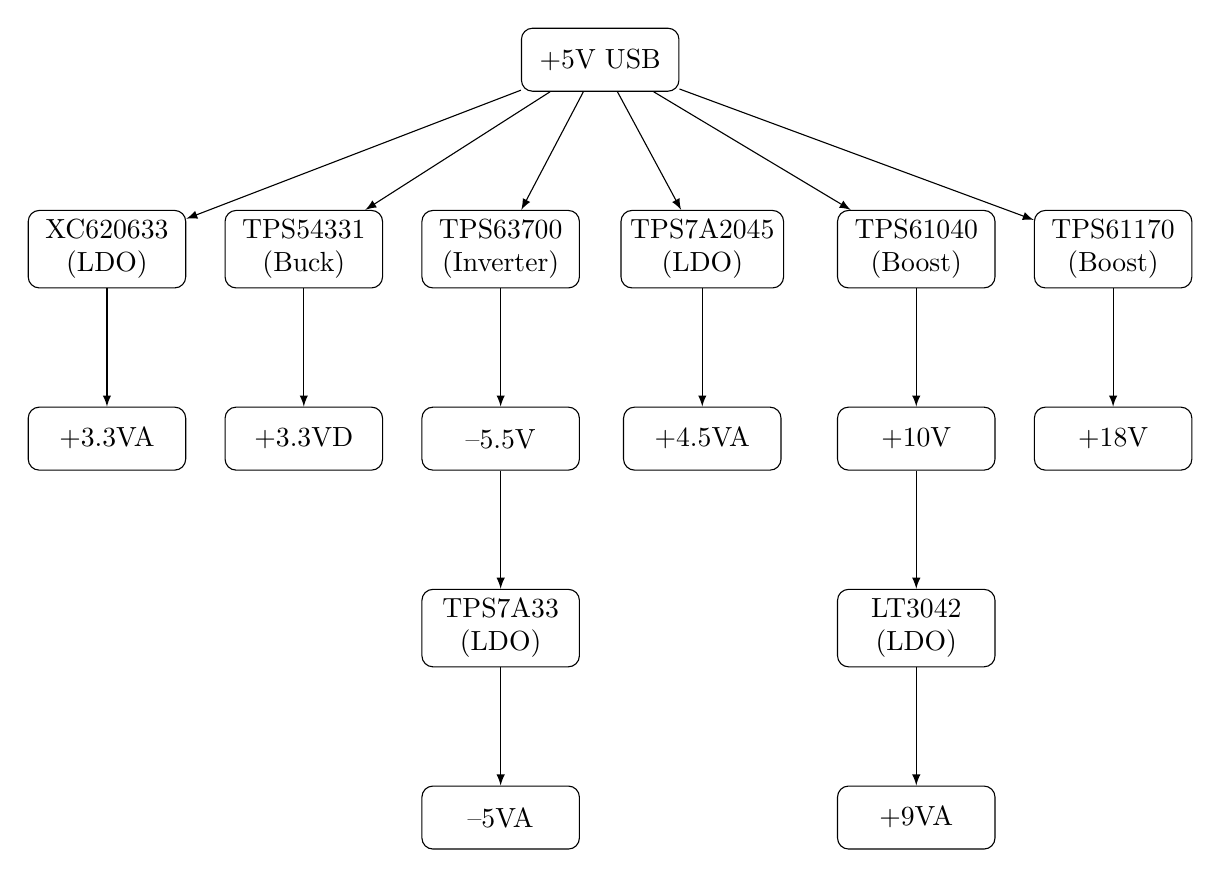
\begin{tikzpicture}[
  rail/.style={draw, rounded corners, minimum width=2cm,
               minimum height=0.8cm, align=center},
  >=latex
]

% Main source
\node[rail] (usb) {+5V USB};

% Branch 1: +3.3VA
\node[rail, below left=1.5cm and 4.25cm of usb] (ldo33) {XC620633\\(LDO)};
\node[rail, below=1.5cm of ldo33] (v33a) {+3.3VA};

% Branch 1: +3.3VD
\node[rail, below left=1.5cm and 1.75cm of usb] (33vd_i) {TPS54331\\(Buck)};
\node[rail, below=1.5cm of 33vd_i] (v33d) {+3.3VD};

% Branch 2: -5VA
\node[rail, below left=1.5cm and -0.75cm of usb] (m55_I) {TPS63700\\(Inverter)};
\node[rail, below=1.5cm of m55_I] (m55) {–5.5V};
\node[rail, below=1.5cm of m55] (ldom5) {TPS7A33\\(LDO)};
\node[rail, below=1.5cm of ldom5] (vm5a) {–5VA};

% Branch 5: +5VA
\node[rail, below right=1.5cm and -0.75cm of usb] (ldop5_i) {TPS7A2045\\(LDO)};
\node[rail, below=1.5cm of ldop5_i] (ldop5) {+4.5VA};

% Branch 4: +9VA
\node[rail, below right=1.5cm and 2cm of usb] (v105_i) {TPS61040\\(Boost)};
\node[rail, below=1.5cm of v105_i] (v105) {+10V};
\node[rail, below=1.5cm of v105] (ldo9) {LT3042\\(LDO)};
\node[rail, below=1.5cm of ldo9] (v9a) {+9VA};

% Branch 3: +18V
\node[rail, below right=1.5cm and 4.5cm of usb] (v18_b) {TPS61170\\(Boost)};
\node[rail, below=1.5cm of v18_b] (v18) {+18V};

% Connections from +5V USB
\draw[->] (usb) -- (ldo33);
\draw[->] (usb) -- (m55_I);
\draw[->] (usb) -- (v18_b);
\draw[->] (usb) -- (v105_i);
\draw[->] (usb) -- (ldop5_i);
\draw[->] (usb) -- (33vd_i);

% Sub-branch arrows
\draw[->] (ldo33) -- (v33a);
\draw[->] (m55) -- (ldom5);
\draw[->] (ldom5) -- (vm5a);
\draw[->] (v105) -- (ldo9);
\draw[->] (ldo9) -- (v9a);
\draw[->] (v18_b) -- (v18);
\draw[->] (m55_I) -- (m55);
\draw[->] (ldop5_i) -- (ldop5);
\draw[->] (v105_i) -- (v105);
\draw[->] (33vd_i) -- (v33d);

\end{tikzpicture}
\caption{Power tree for all the different rail used. Optimized for noise, power efficiency, 
EMI radiation and low BOM}
\label{fig:power_hyerar}
\end{figure}


\begin{table}[htbp]
\small
\setlength{\tabcolsep}{4pt}
\centering
\caption{Estimated current and power budget by rail.}
\label{tab:power-budget}
\begin{tabular}{l l c c c}
\toprule
\textbf{Rail} & \textbf{Part} & \textbf{Current peak (mA)} & \textbf{Power peak (mW)} & \textbf{Power average (mW)} \\
\midrule
+3.3\,V & ESP32-S3-WROOM-1              & 100  & 330  & 70 \\
        & DAN-F10N                      & 19   & 63  & 63 \\
        & microSD (writes)              & 45   & 150  & 5 \\
        & AD7779                        & 15   & 49  & 33  \\
        & MCP4728                       & 1    & 3   & 2 \\
        & ISM330DHCX                    & 5    & 16  & 16 \\
        & TPS62912 ($I_Q$)              & 1    & 3  & 2 \\
        & Misc. (LEDs, logic)           & 5    & 16 & 3 \\
\cmidrule(l){2-5}
        & Subtotal                      & 191  & 617  & \textbf{194} \\
\midrule
+5\,V   & INA851 (3 ch, +$V_\mathrm{s}$)& 10.8  & 54   & 54 \\
        & Offset strap drivers          & 300 & 1500 & 89 (1) \\
\cmidrule(l){2-5}
        & Subtotal                      & 310.8 & 1554 & \textbf{143} \\
\midrule
-5\,V   & INA851 (3 ch, -$V_\mathrm{s}$)& 10.8  & 54   & 54 \\
        & Offset strap drivers          & 300 & 1500 & 89 (1) \\
\cmidrule(l){2-5}
        & Subtotal                      & 310.8 & 1554 & \textbf{143} \\
\midrule
+9\,V   & HMC1001                       & 15  & 135  & 97  \\
        & HMC1002                       & 30  & 270  & 195 \\
\cmidrule(l){2-5}
        & Subtotal                      & 45  & 405 & \textbf{292} \\
\addlinespace
\midrule
\textbf{Total}  &  &  &
\textbf{ } &
\textbf{772 mW} \\
\bottomrule
\end{tabular}
\footnotesize
\raggedright
\textbf{Notes:} (1) The average magnetic field is expected to be \SI{50000}{\nano\tesla}, 
so with an offset constant of \SI{47.5}{\milli\ampere\per\gauss}, if we average all possible field,
we get \SI{35.6}{\milli\ampere} of total average offset current, then we suppose that in average 
the B-field would be split positive and negative.
\vspace{2mm}

\end{table}

\subsubsection{+9V Sensor Bridge Voltage}
To obtain the lowest noise level possible, it is required to first step up the voltage from 
+5V to above the target +9V, then reduce it with a specialized low-noise LDO. The target 
voltage before the LDO is set at +10V to minimize losses while keeping enough headroom to 
guarantee a high PSRR value. To do this, the TPS61040 is selected for being a promotional 
extended part at JLCPCB, which means low price and easy availability; besides this, there 
is no need for any specialized component. Then, the LT3042 is selected to bring this voltage 
down to the desired +9V. This LDO has the advantage of ultra-high PSRR, low spot noise, and 
low RMS noise. 

While doing data transfer, or when not needed, this branch can be turned off using a GPIO of 
the MCU with the TPS61040. A pull-down resistor is added to keep this off until +3.3V is sent 
to the EN pin.

Considering normal operation with three bridge resistances of 850\si{\ohm} giving an equivalent 
of 283.33\si{\ohm}, this results in 32.1~mA and 292~mW in total. With an efficiency of 87\%, the 
TPS61040 will require 73.8~mA at the +5V input.

 \begin{table}[!htbp]
\centering
\caption{+9VA rail: TPS61040 pre-regulator and LT3042 LDO components. (5\,V\,in $\rightarrow$ 
10\,V\, $\rightarrow$ 9\,V\,out)}
\label{tab:9va-bom}
\begin{tabular}{l l l l}
\toprule
\textbf{Stage} & \textbf{Reference} & \textbf{Value} & \textbf{Notes} \\
\midrule
TPS61040 & L1                 & \SI{10}{\micro\henry}        & $\ge\SI{0.6}{A}$ I sat\\
         & D1                 & Schottky, \SI{30}{V}, \SI{0.5}{A} & e.g.\ MBR0530 or equivalent \\
         & $R_{\text{FB1}}$        & \SI{715}{\kilo\ohm}          & $V_{OUT} = 1.233 \cdot 
         \left(1+\frac{R1}{R2}\right)$ \\
         & $R_{\text{FB2}}$        & \SI{100}{\kilo\ohm}          & $\pm\SI{1}{\percent}$ \\
         & $C_{\text{FF}}$         & \SI{22}{\pico\farad}         & \\
         & $C_{\text{IN}}$   & \SI{10}{\micro\farad} $\ge\SI{10}{V}$ &  \\
         & $C_{\text{IN,HF}}$& \SI{100}{\nano\farad} $\ge\SI{10}{V}$ &  \\
         & $C_{\text{OUT}}$  & \SI{10}{\micro\farad} $\ge\SI{25}{V}$ &  \\
         & $C_{\text{OUT,HF}}$ & \SI{100}{\nano\farad} $\ge\SI{25}{V}$ &  \\
         & $R_{\text{EN2}}$        & \SI{100}{\kilo\ohm}          & EN pull-down (MCU control) \\
\midrule
LT3042   & $R_{\text{SET}}$        & \SI{90.9}{\kilo\ohm}         & $ V_{\text{OUT}} = \SI{100}{\micro\ampere} 
         \cdot R_{\text{SET}}$\\
         & $R_{\text{IOUT}}$       & \SI{2}{\kilo\ohm}            & $I_{\text{OUT,max}}(\si{\milli\ampere}) = 
         \frac{125 (\si{\milli\ampere}) \cdot \si{\kilo\ohm}}{R_{\text{IOUT}}}$ \\
         & $C_{\text{SET}}$        & \SI{4.7}{\micro\farad}       &  \\
         & $C_{\text{OUT}}$        & \SI{4.7}{\micro\farad}       &  \\
         & $C_{\text{IN}}$         & \SI{10}{\micro\farad} $\ge\SI{25}{V}$ &  \\
         & $C_{\text{IN,HF}}$      & \SI{100}{\nano\farad} $\ge\SI{25}{V}$ &  \\
\bottomrule
\end{tabular}
\end{table}


\subsubsection{+3.3V Digital}
For the +3.3VD, the TPS54331 is chosen for its very widely availability and being a 
prefered exanded part in JLCPCB. It is able to do up to 3A from 3.5V to 28V input. 
It also has a great efficiency at around 94\%. The table \ref{tab:tps54331_3v3d_webench}
below give the component values for this circuit. This regulator is always on during
normal operation.

\begin{table}[htbp]
\centering
\setlength{\tabcolsep}{16pt}
\caption{TPS54331 +3.3\,V\textsubscript{D} rail (5\,V in $\rightarrow$ 3.3\,V out, $I_\text{out,max}=\SI{0.3}{\ampere}$, WEBENCH values)}
\label{tab:tps54331_3v3d_webench}
\begin{tabular}{lll}
\toprule
\textbf{Ref.} & \textbf{Value} & \textbf{Notes} \\
\midrule
U1      & TPS54331                      & Buck converter, 3\,A, 570\,kHz \\

L1      & \SI{27}{\micro\henry}         & $I_\text{DC}=\SI{1.3}{\ampere}$, $R_\text{DC}=\SI{91}{\milli\ohm}$ \\

D1      & Schottky diode                & $V_\text{RRM}=\SI{20}{\volt}$, $I_\text{O}=\SI{200}{\milli\ampere}$ \\

Cin     & \SI{22}{\micro\farad}, \SI{16}{\volt} 
        & Input bulk capacitor, derated to \SI{16}{\micro\farad} \\
Cout    & \SI{47}{\micro\farad}, \SI{6.3}{\volt} 
        & Output bulk capacitor, derated to \SI{12}{\micro\farad} \\
Cboot   & \SI{100}{\nano\farad}, \SI{10}{\volt} 
        & Bootstrap capacitor (BOOT--PH) \\
Css     & \SI{8.2}{\nano\farad}, \SI{10}{\volt} 
        & Soft–start capacitor \\
Ccomp   & \SI{56}{\nano\farad}, \SI{50}{\volt} 
        & Compensation capacitor (with $R_\text{COMP}$) \\
Ccomp2  & \SI{220}{\pico\farad}, \SI{50}{\volt} 
        & HF pole capacitor in compensation network \\

Rfbt    & \SI{10.2}{\kilo\ohm}, 1\%     & Upper feedback resistor \\
Rfbb    & \SI{3.24}{\kilo\ohm}, 1\%     & Lower feedback resistor, sets $V_\text{OUT}\approx\SI{3.3}{\volt}$ \\
Rcomp   & \SI{4.22}{\kilo\ohm}, 1\%     & Error amplifier compensation resistor \\
\bottomrule
\end{tabular}
\end{table}
\begin{figure}[!htbp]
  \centering
  \includegraphics[width=1\textwidth]{TPS54331.png}
  \caption{Circuit of TPS54331 generated with WEBENCH online tool from TI. The parts are condensend in
  table \ref{tab:tps54331_3v3d_webench}}
  \label{fig:TPS54331}
\end{figure}

\subsubsection{+3.3V Analog}
To reduce the noise level in the ADC, a separate low-noise power line is required. This line 
needs much lower current and lower noise than the +3.3VD. To generate this voltage, the 
XC620633 is chosen. It is a fixed 3.3V LDO with a decent noise level.

\begin{table}[!htbp]
\setlength{\tabcolsep}{30pt}
\centering
\caption{XC620633 +3.3VA rail components (5\,V\,in $\rightarrow$ 3.3\,V\,out)}
\label{tab:xc620633-3v3va-bom}
\begin{tabular}{l l}
\toprule
\textbf{Reference} & \textbf{Value / Part} \\
\midrule
$\text{C}_\text{IN1}$    & 4.7\,\si{\micro\farad}, 10\,V   \\
$\text{C}_\text{IN2}$    & 100\,\si{\nano\farad}, 10\,V    \\
$\text{C}_\text{OUT1}$   & 4.7\,\si{\micro\farad}, 6.3\,V  \\
$\text{C}_\text{OUT2}$   & 100\,\si{\nano\farad}, 6.3\,V   \\
$\text{C}_\text{BULK}$   & 10\,\si{\micro\farad}, 10\,V    \\
\bottomrule
\end{tabular}
\end{table}

\subsubsection{+4.5V Analog}
To get the voltage needed for the INA851 its posisive buffer, a +4.5VA is derived from the
+5V of the USB main supply. The TPS7A2045 is used, this component is a fixed 4.5V LDO witch 
simplify the cicruit while have good noise level. The following table \ref{tab:tps7a2045_4v5va}
gives the passive capacitor values to stabilize the circuit.

\begin{table}[!htbp]
\centering
\setlength{\tabcolsep}{30pt}
\caption{TPS7A2045 +4.5VA rail passive components (5\,V\,in $\rightarrow$ 4.5\,V\,out)}
\label{tab:tps7a2045_4v5va}
\begin{tabular}{ll}
\toprule
\textbf{Ref.}             & \textbf{Value / Part}  \\
\midrule
$\text{C}_\text{IN1}$     & \SI{4.7}{\micro\farad}, \SI{10}{\volt}    \\
$\text{C}_\text{IN2}$     & \SI{0.1}{\micro\farad}, \SI{10}{\volt}    \\
$\text{C}_\text{OUT1}$    & \SI{4.7}{\micro\farad}, \SI{6.3}{\volt}   \\
$\text{C}_\text{OUT2}$    & \SI{0.1}{\micro\farad}, \SI{6.3}{\volt}   \\
\bottomrule
\end{tabular}
\end{table}


\subsubsection{-5V Analog}
To supply the INA851 and the other analog stages with a negative rail, a -5VA is derived from
the +5V USB main supply. First, the TPS63700 is used as an inverting DC/DC converter to
generate an intermediate voltage of approximately -5.5V. This voltage is then regulated by the
low-noise TPS7A33 LDO down to -5V, improving both line rejection and noise performance. The
following table \ref{tab:-5va-bom} summarizes the passive component values used in this design.

\begin{table}[!htbp]
\centering
\caption{-5VA rail: TPS63700 inverting pre-regulator and TPS7A33 LDO components. (5\,V\,in $\rightarrow$ 
-5.5\,V\, $\rightarrow$ -5\,V\,out)}
\label{tab:-5va-bom}
\begin{tabular}{l l l l}
\toprule
\textbf{Stage} & \textbf{Reference} & \textbf{Value} & \textbf{Notes} \\
\midrule
TPS63700 & L1                 & \SI{10}{\micro\henry}       & $\ge\SI{0.6}{A}$ I\textsubscript{sat}, low DCR \\
         & D1                 & Schottky, \SI{20}{V}, \SI{1}{A} & e.g.\ SS14 or equivalent \\
         & $R_{\text{FB1}}$   & \SI{340}{\kilo\ohm}         & Sets $V_{\text{OUT}} \approx \SI{-5.5}{V}$ \\
         & $R_{\text{FB2}}$   & \SI{100}{\kilo\ohm}         & $V_{\text{OUT}} = -1.25 \cdot \left(1+\frac{R_{\text{FB1}}}{R_{\text{FB2}}}\right)$ \\
         & $C_{\text{FF}}$    & \SI{22}{\pico\farad}        & Feed-forward for loop stability \\
         & $C_{\text{IN}}$    & \SI{10}{\micro\farad} $\ge\SI{10}{V}$ & Input bulk capacitor \\
         & $C_{\text{IN,HF}}$ & \SI{100}{\nano\farad} $\ge\SI{10}{V}$ & Input high-frequency bypass \\
         & $C_{\text{OUT}}$   & \SI{10}{\micro\farad} $\ge\SI{10}{V}$ & Output bulk capacitor (inverting node) \\
         & $C_{\text{OUT,HF}}$& \SI{100}{\nano\farad} $\ge\SI{10}{V}$ & Output high-frequency bypass \\
         & $R_{\text{EN}}$    & \SI{100}{\kilo\ohm}         & EN pull-down (MCU control on EN pin) \\
\midrule
TPS7A33  & $C_{\text{IN}}$    & \SI{10}{\micro\farad} $\ge\SI{10}{V}$ & Close to VIN pin, low ESR \\
         & $C_{\text{IN,HF}}$ & \SI{100}{\nano\farad} $\ge\SI{10}{V}$ & HF bypass near VIN/GND \\
         & $C_{\text{OUT}}$   & \SI{10}{\micro\farad} $\ge\SI{10}{V}$ & Output capacitor for stability \\
         & $C_{\text{OUT,HF}}$& \SI{100}{\nano\farad} $\ge\SI{10}{V}$ & HF bypass at VOUT/GND \\
         & $C_{\text{NR}}$    & \SI{10}{\nano\farad}        & Noise-reduction cap on NR pin (if used) \\
\bottomrule
\end{tabular}
\end{table}


\subsubsection{+18V Set/Reset}
To generate the +18V rail, the TPS61288 is chosen. The requirements are not very strict, any source of 
+18V would be able to supply because even if the peak current is very high, about 3.33A, it is only for 
\SI{2}{\micro\second} so the energy is very low. The table \ref{tab:tps61170-bom} shows the chosen 
values for in the schematic of figure \ref{fig:TPS61170}.

\begin{figure}[!htbp]
  \centering
  \includegraphics[width=1\textwidth]{TPS61170.png}
  \caption{Circuit of TPS61170. Taken from the datasheet on p.~9. See table \ref{tab:tps61170-bom} for the 
  componnets values.}
  \label{fig:TPS61170}
\end{figure}

\begin{table}[htbp!]
\centering
\setlength{\tabcolsep}{20pt}
\caption{TPS61170 \SI{18}{V} Boost — Core Schematic Components}
\label{tab:tps61170-bom}
\begin{tabular}{lll}
\toprule
\textbf{Ref} & \textbf{Value / Part} & \textbf{Notes} \\
\midrule
R1 & \SI{137}{k\ohm} & Sets $V_{\text{OUT}}\approx\SI{18.06}{V}$ \\
R2 & \SI{10}{k\ohm} &  see equation  \\
L1 & \SI{10}{\micro\henry}, $I_\text{sat}\ge\SI{1.2}{A}$ & 5$\times$5\,mm class inductor \\
D1 & Schottky, $\ge\SI{40}{V}$ & \\
C1 & \SI{4.7}{\micro\farad}, $\ge\SI{25}{V}$ &  \\
C2 & 4.7–\SI{10}{\micro\farad}, $\ge\SI{25}{V}$ &  \\
R3 & \SI{10}{k\ohm} &  \\
C3 & \SI{680}{pF} &  \\
$\text{R}_{\text{GPIO}}$ & \SI{100}{\ohm}–\SI{1}{k\ohm} & Series from MCU GPIO to CTRL \\
$\text{C}_{\text{CTRL}}$ & 10–\SI{47}{nF} & Small RC on CTRL\\
\bottomrule
\end{tabular}
\end{table}




\end{document}